\chapter{基于国产AI处理器的Top-k算子设计实现}

本文结合国产 AI 处理器的异构计算特点,分析了 Top-k 查询算法的整体运行机制。
具体而言,首先概述了Top-K算法在异构架构下的计算流程。随后,
深入探讨了主机端(CPU)在数据预处理阶段的职责与关键操作。
最后,针对国产 AI 处理器的硬件设计,
详尽阐述了设备端 Top-k 查询算法的实现策略。


\section{国产AI处理器Top-k算子计算流程}
在现代计算领域,随着大数据的迅速发展和人工智能技术的不断进步,
基于国产 AI 芯片的 Top-k 算子计算流程已经逐渐发展为一种典型的异构计算模式,
通常需要主机端(如 CPU)和设备端(如 AI 处理器)协同工作。
整个计算流程可以分为三个主要阶段:数据准备和预处理阶段、数据传输阶段和核心计算阶段。

1. 数据准备和预处理阶段(主机端执行)

在整个Top-k算子计算过程中,数据准备和预处理阶段是非常关键的部分,通常由主机端负责。
在这一阶段,主机端(通常是 CPU)负责接收输入数据,进行格式转换和初步的数据清洗。
由于 AI 处理器通常是为特定任务优化的硬件,其处理能力与 CPU 有很大不同,
因此需要对输入数据进行适配,以确保数据能够适应后续的硬件计算要求。

此外,在这一阶段,主机端还需要对输入进行解析和验证,以确保其合法性和有效性。
这些工作包括检查输入数据的维度、类型,确保数据格式与设备端预期相符等。
在实际应用中,这一阶段的计算量相对较小,但却是整个过程的关键环节,因为如果数据准备不当,
后续计算将无法顺利进行。

2. 数据传输阶段(主机端向设备端传递数据)

数据准备完成后,接下来的步骤是将处理后的数据从主机端传输到设备端(AI 处理器)。
由于 AI 处理器在处理大规模数据时具有极大的并行计算优势,
这一阶段主要是将数据有效地传递到设备端,并确保数据在设备端能够高效地进行计算。
在这一阶段,传输过程的高效性直接影响到整体计算的性能。
如果数据传输时间过长,会影响整个系统的响应时间。
因此,主机端需要选择合适的传输方式,以降低数据传输延迟,确保数据能尽快到达设备端。

3. 核心计算阶段(设备端执行)

核心计算阶段由设备端(AI 处理器)完成,主要任务是根据 Top-k 算子的原理,
利用设备端的硬件特性进行高效的并行计算。在传统的 CPU 环境下,
Top-k 查询算法通常依赖于单线程或少量线程的处理,效率较低。
而在 AI 处理器中,通过硬件的向量化计算指令,可以在多个计算单元上并行执行相同的操作,大大提高计算速度。
因此,设备端的高效计算是整个 Top-k 查询计算流程的核心所在。


综上所述,通过主机端负责数据准备和管理,设备端负责高效计算,
整个计算流程结合了主机端的灵活性和设备端的计算优势,形成了一种典型的异构计算架构。
通过这种分工,能够充分发挥 AI 处理器的硬件优势,提高 Top-k 算法的计算效率。
这一计算流程不仅适用于大规模数据处理,还能够在深度学习和大数据分析等领域得到广泛应用。
图~\ref{fig:topk}展示了该计算流程的具体实现。
\begin{figure}[ht]
    \centering
    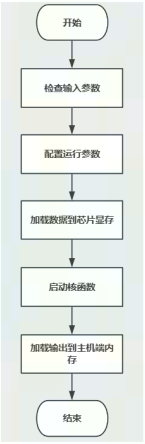
\includegraphics[width=0.3\textwidth]{算子整体流程.png}
    \caption{算子整体流程}
    \label{fig:topk}
    % \note{注:图注的内容不宜放到图题中。}
\end{figure}




\section{主机端数据准备}
    \subsection{接口设计及参数检查}
    拟设计实现的 Top-k 算子输入参数要求如表\ref{tab:input_tab}所示,其中,
    input参数表示输入的张量(tensor),其往往含有多个维度。根据所使用的数据类型,输入张量的元素值可以为整数或浮动小数,
    支持不同的精度(int32 为整数,float32 为浮动小数)。dim 表示待操作的维度,k 表示需要得到的前 k 大/小的值。假设 input 数据总共有 n 个维度,
    并且每个维度的大小为 $\{ x_{0}, x_{1}, \dots, x_{i}, \dots, x_{n-1} \}$,
    则 dim 和 k 所需要满足的数量关系如下:

    \begin{center}
        $0 \leq dim \leq n - 1$
        
        设 dim = i,则: $0 \leq k \leq x_{i}$
    \end{center}
    对于largest,其为bool类型,为true时表示取最大的k个值,为false时,取最小的k个值。
    对于sorted,其为bool类型,为true时表示结果需要排序,为false时,不需要将结果进行排序。
    \begin{table}
        \centering
        \caption{输入参数表}
        \label{tab:input_tab}
        \begin{tabular}{cll} % 注意这里是 'cll' 表示三列,第二列和第三列都对齐左侧
          \toprule
          参数名称   & 数据类型                                       & 描述                          \\
          \midrule
          input & int32/float32 & 输入tensor,可以是任意维度                      \\
          dim & int32   & 表示对第dim维度进行操作            \\
          k   & int32   & 表示取排行前k的数据              \\
          largest & bool   & 默认为true,控制取最大还是最小的值            \\
          sorted & bool   & 默认为false,控制是否需要排序            \\
          
          \bottomrule
        \end{tabular}
    \end{table}

    输出参数表如表\ref{tab:output_tab}所示。其中,
    output是最终的输出 tensor,包含通过 Top-k 查询计算得到的Top-k 大/小值。其数据类型可以是 int32 或 float32,具体取决于输入数据的类型以及计算要求。
    index是与 output 对应的下标。它指示从输入数据的第dim维度的哪个位置获取的 Top-k 元素。
    这在需要返回结果的源数据位置时非常有用,尤其是在需要追踪或处理原始数据时。
    \begin{table}
        \centering
        \caption{输出参数表}
        \label{tab:output_tab}
        \begin{tabular}{cll} % 注意这里是 'cll' 表示三列,第二列和第三列都对齐左侧
          \toprule
          参数名称   & 数据类型                                       & 描述                          \\
          \midrule
          output & /int32/float32 & 输出tensor                 \\
          index   & int32/uint32   & 输出数据在排序维度对应的下标              \\
          \bottomrule
        \end{tabular}
    \end{table}
    

    \subsection{运行参数配置}

        \paragraph{radix-select任务类型}
            需注意的是,radix-selct设备端的并行方案需要多次启动kernel函数,并且需要多核协同完成任务,
            因此每次发起的kernel的任务类型为UnionX。而具体需要多少个core,则根据当前的数据规模来计算得到。
            


        \paragraph{quick-select任务类型}
            quick-select的kernel函数的任务类型为UnionX,X的具体值根据输入数据的大小来进行确定。



\section{设备端Top-k算法实现}
    \subsection{设备端数据摆布方式分析}


Top - K需要支持多维度数据,可以表示如下:\(\text{dim0}\),\(\text{dim1}\),\(\text{dim2}\),
\(\text{dim3}\)。由左到右表示维度从高到低,按照\(\text{dim}\)可以将四个维度转化为:
\(\text{left}\),\(\text{dim}\),\(\text{right}\),\(\text{left}\)为最高维度,
\(\text{dim}\)为中间维度。当\(\text{dim} = 3\)时表示对\(\text{dim3}\)维度进行Top - K查询
,此时\(\text{right} = 1\),\(\text{left} = \text{dim0}×\text{dim1}×\text{dim2}\)。
当\(\text{dim} = 0\)时,表示对\(\text{dim0}\)求Top - K,则对应的\(\text{left}\)和
\(\text{right}\)分别为:\(1\),\(\text{dim1}×\text{dim2}×\text{dim3}\)。

综上所述可以将任意维度的数据抽象成一个三维张量,
其形状为\(\text{left}\),\(\text{dim}\),\(\text{right}\),其中,\(\text{dim}\)是
待操作维度。但是当\(\text{right}≠1\)时,待
操作维度不在最低维,这意味进行数据I/O时,将有可能浪费有限的带宽。因此,在
这种情况下需要针对数据后面两个维度进行转置(transpose)操作。此时张量的形
状为(\(\text{left}\),\(\text{right}\),\(\text{dim}\)),进一步的
,对于Top - k算子而言,其输入的形状可以抽象为(\(\text{left\_right}\),\(\text{dim}\)),
其中\(\text{left\_right}=\text{left}×\text{right}\)。当Top - k任务完成之后,输出的形
状将为(\(\text{left\_right}\),\(\text{k}\)),此时需要对结果再次进行转置操作,其输出形状
为(\(\text{left}\),\(\text{k}\),\(\text{right}\)),
作为最终Top - k算子的最终结果。其形状的转变流程如图~\ref{fig:input_shape}

\begin{figure}[ht]
    \centering
    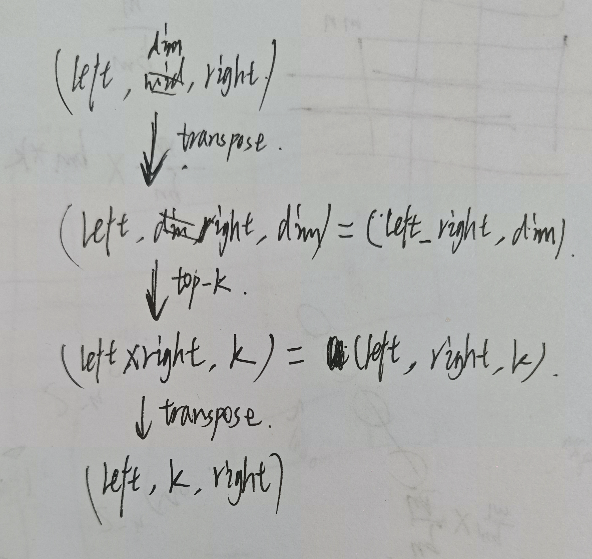
\includegraphics[scale = 0.4]{input_shape.png}
    \caption{}
    \label{fig:input_shape}
    % \note{注:图注的内容不宜放到图题中。}
\end{figure}



    \subsection{quick-select Top-k算子实现}
    并行选择算法的核心目标是找到输入数组\(A = [a_{1}, a_{2},\cdots, a_{n}]\)中的第\(k\)大或第\(k\)小元素。该问题通过构造子数组\(L\)和\(R\)并递归地缩小问题规模来求解。
    完整算法的伪代码如算法~\ref{alg:quick_select}所示。
    
    
    \begin{algorithm}
        \SetAlgoLined
        \KwIn{Array $A$ with $n$ entries, integer $k \leq n$}
        \KwOut{Value of the $k$th largest element in $A$}
        $p \leftarrow$ a value selected uniformly at random from $A$ \tcp{This is our pivot.}
        $L \leftarrow$ elements in $A$ which are less than pivot $p$ \tcp{Requires $\Theta(n)$ work}
        $R \leftarrow$ elements in $A$ which are larger than pivot $p$\\
        \If{$|L|$ is $k - 1$}{
            \Return $p$ \tcp{The pivot itself is the $k$th largest element}
        }
        \If{$|L| > k$}{
            \Return \textproc{Select($L$, $k$)} \tcp{$k$th largest element lives in $L$}
        }
        \Else{
            \Return \textproc{Select($R$, $k - |L| - 1$)} \tcp{$k$th largest element lives in $R$}
        }
        \caption{Select(A, k)}
        \label{alg:quick_select}
    \end{algorithm}

    其算法流程描述如下:

    \begin{itemize}
        \item \textbf{选择枢轴:}  
        算法从输入数组 $A$ 中随机选择一个枢轴 $p$。该过程可以视为划分操作的起点。
        
        \item \textbf{划分数组:}  
        根据枢轴 $p$,将数组 $A$ 分为两个子数组:
        \begin{itemize}
            \item $L$:存储小于 $p$ 的元素;
            \item $R$:存储大于或等于 $p$ 的元素。
        \end{itemize}
        划分操作的计算复杂度为 $O(n)$,其中每次递归需要处理的数组规模依次减小,从而逐步缩小问题规模。
    
        \item \textbf{递归求解:}  
        \begin{itemize}
            \item 如果 $k$ 恰好对应 $p$ 的位置,直接返回 $p$;
            \item 如果 $k$ 小于子数组 $L$ 的大小,则递归处理 $L$;
            \item 否则,递归处理 $R$,并更新 $k$ 的值以反映当前查找范围的变化。
        \end{itemize}
 
    \end{itemize}



    
    
    
    在并行选择算法中,数组划分(Partitioning)是关键步骤,其性能对整体算法的效率有显著影响。划分操作的目标是依据选定的枢轴(pivot),将输入数组\(A = [a_{1}, a_{2},\cdots, a_{n}]\)分为两个子集:

\(L = \{x \mid x < pivot\}\),即所有小于枢轴的元素集合。

\(R = \{x \mid x \geq pivot\}\),即所有大于或等于枢轴的元素集合。

在传统的串行实现中,划分操作通过逐一扫描数组完成,其时间复杂度为\(O(n)\)。
然而,这种方法在并行环境中难以充分利用多处理器的计算资源。
为此,本文通过引入前缀和(PrefixSum)技术,对划分操作进行并行化优化。
算法伪代码如算法~\ref{alg:Construct}:

\begin{algorithm}
    \SetAlgoLined
    Allocate and empty array of size $n$, with all values initially 0.\;
    Construct indicator list $B_L[0,\ldots,n - 1]$, where $b_i = 1\{a_i < p\}$\;
    Compute PrefixSum on $B_L$ \tcp{This requires $O(\log n)$ depth}
    Create the array $L$ of size $\text{PrefixSum}(B_L)[n - 1]$ \;
    \For{$i = 1,2,\ldots,n$}{
      $L[\text{PrefixSum}(B_L)[i]] \leftarrow a_i$ \tcp{Can be done in parallel}
    }
    \caption{ Constructing $L$ (or $R$)}
    \label{alg:Construct}
  \end{algorithm}

  \paragraph{步骤详解}

1. 构建标记数组

为了实现划分操作,首先对输入数组\(A\)构造一个标记数组\(B\),其定义如下:
\[
B[i]=
\begin{cases}
1, & \text{若 } a_{i}<pivot\\
0, & \text{若 } a_{i}\geq pivot
\end{cases}
\]

标记数组\(B\)的每个元素表示输入数组\(A\)中对应位置的元素是否属于\(L\)。构建\(B\)的过程可以在并行环境中高效完成,因为每个处理器只需独立判断若干元素的条件。
例如,给定输入数组\(A = [3,7,2,5,6]\),若枢轴为\(pivot = 5\),则标记数组\(B=[1,0,1,0,0]\)。

2. 计算前缀和

在获得标记数组\(B\)后,计算其前缀和数组\(P\),定义如下:
\[
P[i]=\sum_{j = 1}^{i}B[j]
\]

其中\(P[i]\)表示在标记数组\(B\)中从第\(1\)个到第\(i\)个元素中值为\(1\)的元素个数。前缀和计算可以使用并行扫描(Parallel Scan)技术完成,其时间复杂度为\(O(\log n)\)。
继续以上示例,对\(B = [1,0,1,0,0]\)计算前缀和:
\[
P=[1,1,2,2,2]
\]

3. 确定目标位置

通过前缀和数组\(P\),可以快速确定每个元素在目标数组\(L\)或\(R\)中的位置:
\begin{itemize}
    \item 若\(B[i] = 1\)(即\(a_{i}<pivot\)),则\(a_{i}\)属于\(L\),其在\(L\)中的位置为\(P[i] - 1\)。
    \item 若\(B[i] = 0\)(即\(a_{i}\geq pivot\)),则\(a_{i}\)属于\(R\),其位置可以通过全局计数和前缀和计算确定。
\end{itemize}

4. 构造$L$($R$)

 根据前缀和数组\(P\),将A中的元素赋值到$L$($R$)指定位置,此操作为一个Scatter操作,可以并行执行。
继续以上示例:
\begin{itemize}
    \item 元素\(3\)(\(B[1]=1\))在\(L\)中的位置为\(P[1] - 1 = 0\);
    \item 元素\(7\)(\(B[2]=0\))在\(R\)中的位置为\(\vert L\vert+\text{当前}(R\text{的偏移量})\)。
\end{itemize}




\paragraph{并行实现}

在并行实现中,划分操作分以下几步:
\begin{enumerate}
    \item 使用多个处理器计算标记数组\(B\),每个处理器负责数组的一部分。
    \item 使用并行扫描技术计算前缀和\(P\),其时间复杂度为\(O(\log n)\)。
    \item 根据前缀和数组\(P\),每个处理器独立将元素从输入数组\(A\)复制到目标数组\(L\)或\(R\)。
\end{enumerate}
     
\subparagraph{选择pivot}


\subparagraph{构建L(R)}


\subsection{radix-select Top-k算子实现}
基数选择(radix-select)是基数排序的一种应用,用于在一组数据中找到具有特定排名的元素。
它通过在基数排序的过程中,只对包含目标元素的分区进行递归操作,从而减少不必要的计算。
在radix-select top - \(K\)算法中,一个数位(digit)对应着一个元素二进制表示中
的一组连续的\(b\)位。该算法从最高有效数位(most significant digit)到最低有效
数位(least significant digit)处理一个元素,每次迭代处理一个数位。
对于一个由\(r\)位组成的元素,需要进行\(\lceil\frac{r}{b}\rceil\)次迭代。每次迭代主要包含四步,
其伪代码见算法~\ref{alg:Counting}。

\begin{algorithm}
    \SetAlgoLined
    \KwIn{Array $D$ with $n$ entries, integer $k \leq n$}
    \KwOut{array R is the Top-k elements}
    $Bucket \leftarrow$ init $0$ \tcp{size is $2^{digit}$}\\ 
    \underline{HISTOGRAM - KEYS}\\
    \For{$j \leftarrow 0$ to $N - 1$}{
      $Bucket[D[j]] \leftarrow Bucket[D[j]] + 1$
    }
    \underline{SCAN - BUCKETS}\\
    $Sum \leftarrow 0$\\
    \For{$i \leftarrow 0$ to $2^r - 1$}{
      $Val \leftarrow Bucket[i]$ \\
      $Bucket[i] \leftarrow Sum$ \\
      $Sum \leftarrow Sum + Val$ \\
    }
    \underline{FIND TARGET BUCKET}\\
    \For{$i \leftarrow 0$ to $2^r - 1$}{
        \If{Bucket[i] \ge k}{\\
            $POS \leftarrow Bucket[i]$\\ 
            break;\\
        }\\
    }
    \underline{FILTER}\\
    \For{$j \leftarrow 0$ to $N - 1$}{
        If{ D[j] \ge POS}{
            continue;
          }\\

        
    $A \leftarrow Bucket[D[j]]$ \\

      $R[A] \leftarrow K[j]$ \\

      $Bucket[D[j]] \leftarrow A + 1$\\
    }
    \caption{Counting - Sort Algorithm}
    \label{alg:Counting}
  \end{algorithm}
  
  算法原理
  类比于 Quicksort 中的 Quickselect,RadixSelect 算法过程与基数排序算法相似,
  与之不同的是,其在迭代的过程中,RadixSelect仅对包含第 k 大元素的数进行基数排序,达到减少问题规模的效果。
 
  \paragraph{步骤详解}

 ### 1. 初始化桶

  首先,需要初始化一个名为\(Bucket\)的数组,其大小设置为\(2^{digit}\),并且将数组中的所有元素初始化为\(0\)。其中digit为读取数据的位数,这个\(Bucket\)数组的主要作用是用于统计数组\(D\)中每个元素出现的次数。
  
  ### 2. 构建直方图

 在此阶段,会遍历数组\(D\)中的每一个元素\(D[j]\),统计\(D[j]\)中元素出现的个数,记录在\(Bucket\)中。
  
 ### 3. 扫描桶

 计算出每个桶的累积和,而这个累积和对于确定每个元素在排序后的位置起到了关键作用。

  ### 4. 找到目标桶

再次遍历\(Bucket\)数组,目的是找到第一个满足\(Bucket[i] \geq k\)的桶。

  ### 5. 过滤

  在此阶段,会再次遍历数组\(D\),目的是将数组\(D\)中的前\(k\)大元素挑选出来,
  并放入结果数组\(R\)中。

  上述串行算法由于在所有阶段都存在循环依赖关系,所以不能直接并行化(或向量化)。
  如果试图对"构建直方图"(HISTOGRAM - KEYS)的迭代进行并行处理,可能会有多个处理器同时尝试
  对同一个桶(bucket)进行递增操作,产生资源竞争。而如果锁定桶,当有许多键具有相同数位时,
  桶将成为串行瓶颈,将会极大地降低性能。

  基于以上的分析,可以通过为每个处理器分配一组独立的桶(本地桶),
进而在不需要对桶进行锁定的情况下实现算法并行化:
即每个处理器负责其自己的局部数据(\(\frac{N}{P}\)子集),
并将它们列入自己的本地桶集合中。
此时,可以将所有的桶看作是一个矩阵\(Buckets[i, j]\),如下图~\ref{fig:process_bucket}:

\begin{figure}[ht]
    \centering
    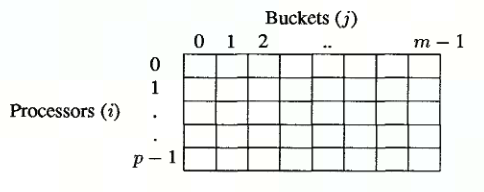
\includegraphics[scale = 0.6]{process_bucket.png}
    \caption{}
    \label{fig:process_bucket}
    % \note{注:图注的内容不宜放到图题中。}
\end{figure}

其中 $i$ 是处理器数,$j$ 是本地桶的桶数。在每个处理器都拥有自己的桶之后,
每个处理器在进行基数选择的
第一阶段,第三阶段和第四阶段(HISTOGRAMKEYS , FIND TARGET BUCKET和 FILTER)时,
都在自己的局部数据上进行工作,从而解除所有依赖项。
但需要注意到,为了保证结果的正确性,第三阶段( SCAN-BUCKETS )将必须进行修改。因为如果
每个处理器仅扫描自己的本地桶,将仅仅只能得到局部数据的Top-k结果,导致结果错误。而通过分析我们发现,
$Buckets[i][j]$代表在进行SCAN-BUCKETS处理后,$A$中元素最终在结果$R$中的偏移位置,
具体关系见下图~\ref{fig:digits}:
\begin{figure}[ht]
    \centering
    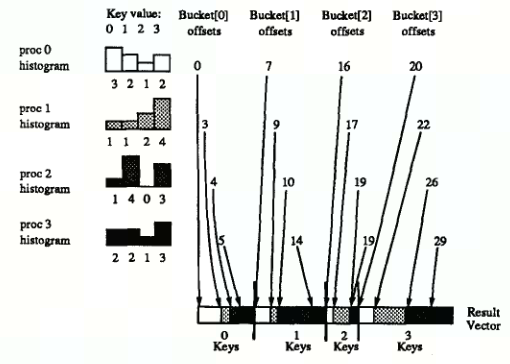
\includegraphics[scale = 0.6]{process_digits.png}
    \caption{并行radix-select的扫描步骤}
    \label{fig:digits}
    % \note{注:图注的内容不宜放到图题中。}
\end{figure}

假如该算法用 4 个处理器和 4 个桶来对 0 - 3 的值进行排序。偏移量是通过扫描桶来计算的。
扫描之后,每个处理器在具有特定值的键的最终输出中都有一个起始位置。
例如,处理器 3 将把值为 “0” 的键从输出中的第 5 个位置开始放置,把值为 “1” 的键从第 14 个位置开始放置,如偏移量所示。

所以需要将矩阵\(Buckets[i, j]\)在列方向上以及行方向上进行扫描操作,以汇总全局信息,
其数学公式见~\ref{equ:buckets}
\begin{equation}
    \text{ Buckets}[i, j]' = \sum_{k = 0}^{p - 1} \sum_{m = 0}^{j - 1} \text{ Buckets}[k, m] + \sum_{k = 0}^{i - 1} \text{ Buckets}[k, j]
    \label{equ:buckets}
\end{equation}
也就是说,偏移量是所有处理器中小于 $j$ 的数位总数,再加上小于 $i$ 的处理器中数位等于 $j$ 的数量。
这个总和可以通过将$Buckets$矩阵按列优先顺序展开,
然后对展开后的矩阵执行 “SCAN - BUCKETS” 操作来进行计算。
%   在并行实现中,划分操作分以下几步:
%   \begin{enumerate}
%       \item 使用多个处理器计算标记数组\(B\),每个处理器负责数组的一部分。
%       \item 使用并行扫描技术计算前缀和\(P\),其时间复杂度为\(O(\log n)\)。
%       \item 根据前缀和数组\(P\),每个处理器独立将元素从输入数组\(A\)复制到目标数组\(L\)或\(R\)。
%   \end{enumerate}
\paragraph{并行实现}
\subparagraph{初始化桶}

首先,需要初始化一个名为\(Bucket\)的数组,其大小设置为\(2^{digit}\),并且将数组中的所有元素初始化为\(0\)。其中digit为读取数据的位数,这个\(Bucket\)数组的主要作用是用于统计数组\(D\)中每个元素出现的次数。
\subparagraph{构建直方图}

在此阶段,会遍历数组\(D\)中的每一个元素\(D[j]\),统计\(D[j]\)中元素出现的个数,记录在\(Bucket\)中。
\subparagraph{扫描桶}

计算出每个桶的累积和,而这个累积和对于确定每个元素在排序后的位置起到了关键作用。

\subparagraph{找到目标桶}

再次遍历\(Bucket\)数组,目的是找到第一个满足\(Bucket[i] \geq k\)的桶。
\subparagraph{过滤}

在此阶段,会再次遍历数组\(D\),目的是将数组\(D\)中的前\(k\)大元素挑选出来,
并放入结果数组\(R\)中。





  
\section{本章小结}
